\section{Controle por realimentação de estados}

\begin{frame}{Controlabilidade}
\begin{block}{Definição}
O par $(A,B)$, $A \in \mathbb{R}^{n \times n}$, $B \in \mathbb{R}^{n \times r}$ é \textbf{controlável} se para todo $\bm{x}_0$ e $\bm{x}_1$ existe a sequência de sinais de controle $\bm{u}(0)$, $\bm{u}(1)$, $\cdots$, $\bm{u}(N)$, $\bm{u}(k) \in \mathbb{R}^{r}$ para $N \in \mathbb{Z}$ finito tal que se o estado do sistema for $\bm{x}_0$ em $k = 0$, o mesmo será forçado pelo sinal de controle para $\bm{x}_1$ em $k \leq N$.
\end{block}
\end{frame}

\begin{frame}{Controlabilidade}
\begin{block}{Definição}
\begin{itemize}
    \item Em outras palavras, o sistema é dito \textbf{controlável} se for possível \textbf{transferir o sistema de qualquer estado inicial arbitrário a qualquer estado desejado} (também um estado arbitrário) em um período de tempo finito; ou seja, se cada variável de estado puder ser controlada em um período de tempo finito por algum sinal de controle não sobrecarregado.
    \item Se qualquer \textbf{variável de estado é independente do sinal de controle}, então é impossível controlar esta variável de estado e, portanto, o sistema é \textbf{incontrolável}.
\end{itemize}
\end{block}
\end{frame}

\begin{frame}{Controlabilidade}
\begin{block}{Solução da equação dinâmica}
\begin{itemize}
    \item A partir de 
\end{itemize}
$$\bm{x}(k+1) = A\bm{x}(k) + B\bm{u}(k)$$
\begin{align*}
    \bm{x}(1) &= A\bm{x}(0) + B\bm{u}(0) \\
    \bm{x}(2) &= A\bm{x}(1) + B\bm{u}(1) = A[A\bm{x}(0) + B\bm{u}(0)] + B\bm{u}(1) \\
    &= A^2\bm{x}(0) + AB\bm{u}(0) + B\bm{u}(1) \\
    \bm{x}(3) &= A\bm{x}(2) + B\bm{u}(2) = A[A^2\bm{x}(0) + AB\bm{u}(0) + B\bm{u}(1)] + B\bm{u}(2) \\
    &= A^3\bm{x}(0) + A^2B\bm{u}(0) + AB\bm{u}(1) + B\bm{u}(2) \\
    \vdots  \\
    \bm{x}(k) &= A^k\bm{x}(0) + \sum_{n=0}^{k-1} A^n B\bm{u}(k-1-n) = A^k\bm{x}(0) + \sum_{n=0}^{k-1} A^{k-1-n} B\bm{u}(n)
\end{align*}
\end{block}
\end{frame}

\begin{frame}{Controlabilidade}
\begin{block}{Solução da equação dinâmica}
\begin{itemize}
    \item Portanto, podemos escrever:
\end{itemize}
\begin{align*}
    \bm{x}(N) &= A^N\bm{x}(0) + \sum_{n=0}^{N-1} A^{N-1-n} B\bm{u}(n) \\
    &= A^N\bm{x}(0) + \begin{bmatrix} B & AB & A^2B & \cdots & A^{N-1}B \end{bmatrix}
    \begin{bmatrix} \bm{u}(N-1) \\ \vdots \\ \bm{u}(0) \end{bmatrix}
\end{align*}
\vspace{-0.3cm}
\begin{itemize}
    \item Como o estado no instante $N$ deve ser $\bm{x}_1$ e  chamando a condição inicial de $\bm{x}_0$, temos o  sistema de $n$ equações que deve ter solução para que o sistema seja controlável:
\end{itemize}
\vspace{-0.4cm}
\begin{align*}
    \bm{x}_1 - A^N\bm{x}_0 = \begin{bmatrix} B & AB & A^2B & \cdots & A^{N-1}B \end{bmatrix}
    \begin{bmatrix} \bm{u}(N-1) \\ \vdots \\ \bm{u}(0) \end{bmatrix}
\end{align*}
\end{block}
\end{frame}

\begin{frame}{Controlabilidade}
\begin{block}{Teorema da controlabilidade}
\begin{itemize}
    \item A equação anterior é um sistema de equações lineares da forma $\beta = \mathcal{C} \alpha$, onde $\beta$ e $\mathcal{C}$ são conhecidos.
    \item Se o sistema for controlável, então existe  uma sequência finita de controle $\bm{u}(k), \ k =  0, 1, \cdots, N-1$ que leva o estado de $\bm{x}_0$ a $\bm{x}_1$. Em outras palavras, \textbf{o sistema de equações deve ter solução}.
    \item Para que o sistema de equações tenha solução é necessário e suficiente que a  matriz $\mathcal{C}$ (\textit{matriz de controlabilidade}) tenha \textbf{posto} $\bm{n}$ (\textit{seja não singular}), isto é, ela deve ter $\bm{n}$ \textbf{linhas ou colunas linearmente independentes}.
\end{itemize}
$$\boxed{\rho[\mathcal{C}] = n}$$
\end{block}
\end{frame}

\begin{frame}{Controlabilidade}
\begin{block}{Teorema da controlabilidade}
\begin{itemize}
    \item Uma forma usual e prática de verificar a controlabilidade (\textit{principalmente para sistemas de ordem elevada}) é garantir que \textbf{o determinante da matriz de controlabilidade seja diferente de zero} (\textit{se você não sabe álgebra linear terá de aceitar essa afirmação na base da fé}).
    \item Deve ser notado que a controlabilidade de estado \textbf{independe da saída}.
\end{itemize}
\end{block}
\end{frame}

\begin{frame}{Controlabilidade}
\begin{block}{Exemplo físico}
	Devido à simetria do circuito, não é possível, manipulando a fonte de tensão  $u$, alterar a tensão sobre capacitor, que é a  variável de estado do circuito. 
\end{block}
\centerline{\includegraphics[width=0.4\linewidth]{Figuras/Ch15/fig0.PNG}}
\end{frame}

\begin{frame}{Controlabilidade - Exemplo \#01}
\begin{block}{Problema}
Verificar se o sistema abaixo é completamente controlável.
\begin{align*}
    \begin{bmatrix} x_1(k+1) \\ x_2(k+1) \end{bmatrix}
    &=
    \begin{bmatrix}
    0 & 1 \\ -2 & 3
    \end{bmatrix}
    \begin{bmatrix}
    x_1(k) \\ x_2(k)
    \end{bmatrix}
    +
    \begin{bmatrix}
    0 \\ 1
    \end{bmatrix}
    u(k)
\end{align*}
\end{block}
\end{frame}

\begin{frame}{Controlabilidade - Exemplo \#01}
\begin{block}{Resolução}
\begin{itemize}
    \item A matriz de controlabilidade é dada por:
\end{itemize}
\begin{align*}
    \mathcal{C} &= \begin{bmatrix} B & AB \end{bmatrix} \\
    &= \begin{bmatrix} 0 & 1 \\ 1 & 3 \end{bmatrix}
\end{align*}
\vspace{-0.3cm}
\begin{itemize}
    \item Calculando o determinante da matriz de controlabilidade, temos:
\end{itemize}
$$\text{det}[\mathcal{C}] = -1 \neq 0 $$
Desta forma, o sistema é completamente controlável e $\rho = n = 2$.
\end{block}
\end{frame}

\cprotect\frame{
\frametitle{\MATLAB}
\begin{block}{}
\begin{verbatim}
>>ctrb(A,B) 
\end{verbatim}
computa a matriz de controlabilidade representada pelo par $\bm{(A,B)}$. \\
\vspace{0.2cm}
\textbf{Exemplo}: cálculo do exemplo \#01
\end{block}
\centerline{\includegraphics[width=0.3\linewidth]{Figuras/Ch15/fig1.PNG}}
}

\begin{frame}{Controlabilidade - Exemplo \#02}
\begin{block}{Problema}
Verificar se o sistema descrito pelo diagrama de fluxo de sinal mostrado abaixo é completamente controlável.
\end{block}
\centerline{\includegraphics[width=0.85\linewidth]{Figuras/Ch15/fig2.PNG}}
\end{frame}

\begin{frame}{Controlabilidade - Exemplo \#02}
\begin{block}{Resolução}
\begin{itemize}
    \item A equação dinâmica, de acordo com o diagrama de fluxo de sinal, pode ser escrita como:
\end{itemize}
\begin{align*}
    \begin{bmatrix} x_1(k+1) \\ x_2(k+1) \end{bmatrix}
    &=
    \begin{bmatrix}
    a_2 & 1 \\ 0 & a_1
    \end{bmatrix}
    \begin{bmatrix}
    x_1(k) \\ x_2(k)
    \end{bmatrix}
    +
    \begin{bmatrix}
    1 \\ 0
    \end{bmatrix}
    u(k)
\end{align*}
\end{block}
\end{frame}

\begin{frame}{Controlabilidade - Exemplo \#02}
\begin{block}{Resolução}
\begin{itemize}
    \item A matriz de controlabilidade é dada por:
\end{itemize}
\begin{align*}
    \mathcal{C} &= \begin{bmatrix} B & AB \end{bmatrix} \\
    &= \begin{bmatrix} 1 & a_2 \\ 0 & 0 \end{bmatrix}
\end{align*}
\vspace{-0.3cm}
\begin{itemize}
    \item Calculando o determinante da matriz de controlabilidade, temos:
\end{itemize}
$$\text{det}[\mathcal{C}] = 0 $$
Desta forma, o sistema não é completamente controlável pois $\rho = 1 \neq n = 2$ (\textit{presença de uma linha linearmente dependente}).
\begin{itemize}
    \item Esse resultado era esperado, uma vez que pelo diagrama de fluxo de sinal pode ser visto que a entrada $u(k)$ não afeta o  estado $x_2(k)$. Geometricamente isso significa que há regiões no espaço de estado (\textit{o subespaço não controlável}) para onde não é possível levar o sistema (o estado $\bm{x}$) em tempo finito por meio da ação de controle $u(k)$.
\end{itemize}
\end{block}
\end{frame}

\begin{frame}{Observabilidade}
\begin{block}{Definição}
O par $(A,C)$, $A \in \mathbb{R}^{n \times n}$, $C \in \mathbb{R}^{p \times n}$ é \textbf{observável} se para qualquer $\bm{x}_0$, essa condição inicial pode ser determinada a partir da sequência finita de valores $\bm{y}(0)$, $\bm{y}(1)$, $\cdots$, $\bm{y}(N-1)$, $\bm{y}(k) \in \mathbb{R}^{p}$, e de entradas $\bm{u}(0)$, $\bm{u}(1)$, $\cdots$, $\bm{u}(N-1)$, $\bm{u}(k) \in \mathbb{R}^{r}$, para $N \in \mathbb{Z}$ finito.
\end{block}
\end{frame}

\begin{frame}{Observabilidade}
\begin{block}{Definição}
\begin{itemize}
    \item No caso de observabilidade, diz-se que o estado de uma planta é \textbf{observável} se qualquer que seja seu valor inicial $\bm{x}_0$, o mesmo  pode ser determinado a partir de medidas do sinal de saída $\bm{y}$ e de entrada (se houver) $\bm{u}$ tomadas durante um intervalo finito de tempo.
\end{itemize}
\end{block}
\end{frame}

\begin{frame}{Observabilidade}
\begin{block}{Solução da equação de saída}
\begin{itemize}
    \item A partir de 
\end{itemize}
$$\bm{y}(k) = C\bm{x}(k) + D\bm{u}(k)$$
\begin{align*}
    \bm{y}(0) &= C\bm{x}(0) + D\bm{u}(0) \\
    \bm{y}(1) &= C\bm{x}(1) + D\bm{u}(1) = C[A\bm{x}(0) + B\bm{u}(0)] + D\bm{u}(1) \\
    &= CA\bm{x}(0) + CB\bm{u}(0) + D\bm{u}(1) \\
    \bm{y}(2) &= C\bm{x}(2) + D\bm{u}(2) = C[A^2\bm{x}(0) + AB\bm{u}(0) + B\bm{u}(1)] + D\bm{u}(2) \\
    &= CA^2\bm{x}(0) + CAB\bm{u}(0) + CB\bm{u}(1) + D\bm{u}(2) \\
    \vdots  \\
    \bm{y}(N-1) &= CA^{N-1}\bm{x}(0) + \sum_{n=0}^{N-2} CA^{N-2-n} B\bm{u}(n) + D\bm{u}(N-1)
\end{align*}
\end{block}
\end{frame}

\begin{frame}{Observabilidade}
\begin{block}{Solução da equação de saída}
\begin{itemize}
    \item Na forma matricial, temos:
\end{itemize}
\begin{align*}
\begin{bmatrix}
    \bm{y}(0) - D\bm{u}(0) \\
    \bm{y}(1) - CB\bm{u}(0) - D\bm{u}(1) \\
    \vdots  \\
    \bm{y}(N-1) - \sum_{n=0}^{N-2} CA^{N-2-n} B\bm{u}(n) - D\bm{u}(N-1)
\end{bmatrix}
=
\begin{bmatrix}
C \\
CA \\
\vdots \\
CA^{N-1}
\end{bmatrix}
\bm{x}(0)
\end{align*}
\end{block}
\end{frame}

\begin{frame}{Observabilidade}
\begin{block}{Teorema da observabilidade}
\begin{itemize}
    \item A equação anterior é um sistema de equações lineares da forma $\beta = \mathcal{O} \alpha$, onde $\beta$ e $\mathcal{O}$ são conhecidos.
    \item A mesma análise realizada para o problema de controlabilidade pode ser realizada aqui. Assim, é possível determinar $\bm{x}(0)$ unicamente se houver $\bm{n}$ \textbf{equações linearmente independentes}.
    \item Para que o sistema de equações tenha solução é necessário e suficiente que a  matriz $\mathcal{O}$ (\textit{matriz de observabilidade}) tenha \textbf{posto} $\bm{n}$ (\textit{seja não singular}), isto é, ela deve ter $\bm{n}$ \textbf{linhas ou colunas linearmente independentes}.
\end{itemize}
$$\boxed{\rho[\mathcal{O}] = n}$$
\end{block}
\end{frame}

\begin{frame}{Observabilidade}
\begin{block}{Teorema da observabilidade}
\begin{itemize}
    \item Uma forma usual e prática de verificar a observabilidade (\textit{principalmente para sistemas de ordem elevada}) é garantir que \textbf{o determinante da matriz de observabilidade seja diferente de zero} (\textit{se você não sabe álgebra linear terá de aceitar essa afirmação na base da fé}).
    \item Quando o estado não é mensurável, é impossível a implementação deste tipo de controle. Porém, é possível obter uma estimativa do vetor $\bm{x}$, usando apenas os sinais de entrada, $\bm{u}$, e de saída, $\bm{y}$, que são sempre mensuráveis. \textbf{O esquema que estima o estado a partir da entrada e da saída é denominado de observador de estado}.
\end{itemize}
\end{block}
\end{frame}

\begin{frame}{Observabilidade - Exemplo \#01}
\begin{block}{Problema}
Verificar se o sistema representado pelo diagrama de simulação abaixo é completamente observável.
\end{block}
\vspace{0,4 cm}
\centering
\scalebox{.65}{


\tikzset{every picture/.style={line width=0.75pt}} %set default line width to 0.75pt        

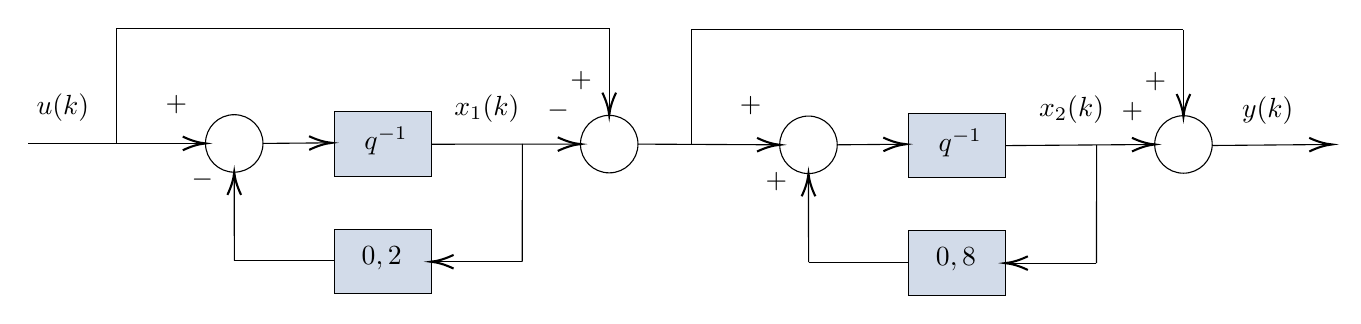
\begin{tikzpicture}[x=0.75pt,y=0.75pt,yscale=-1,xscale=1]
%uncomment if require: \path (0,300); %set diagram left start at 0, and has height of 300

%Straight Lines [id:da6568557179723491] 
\draw    (601.03,101.15) -- (656.73,100.67) ;
\draw [shift={(658.73,100.65)}, rotate = 539.5] [color={rgb, 255:red, 0; green, 0; blue, 0 }  ][line width=0.75]    (10.93,-3.29) .. controls (6.95,-1.4) and (3.31,-0.3) .. (0,0) .. controls (3.31,0.3) and (6.95,1.4) .. (10.93,3.29)   ;
%Shape: Circle [id:dp5521138985171623] 
\draw  [color={rgb, 255:red, 0; green, 0; blue, 0 }  ,draw opacity=1 ] (116,100.15) .. controls (116,92.5) and (122.2,86.3) .. (129.85,86.3) .. controls (137.5,86.3) and (143.7,92.5) .. (143.7,100.15) .. controls (143.7,107.8) and (137.5,114) .. (129.85,114) .. controls (122.2,114) and (116,107.8) .. (116,100.15) -- cycle ;
%Straight Lines [id:da4237274960130786] 
\draw [color={rgb, 255:red, 0; green, 0; blue, 0 }  ,draw opacity=1 ]   (129.9,156.65) -- (177.9,156.65) ;
%Straight Lines [id:da109487651456454] 
\draw [color={rgb, 255:red, 0; green, 0; blue, 0 }  ,draw opacity=1 ]   (129.9,156.65) -- (129.85,116) ;
\draw [shift={(129.85,114)}, rotate = 449.93] [color={rgb, 255:red, 0; green, 0; blue, 0 }  ,draw opacity=1 ][line width=0.75]    (10.93,-3.29) .. controls (6.95,-1.4) and (3.31,-0.3) .. (0,0) .. controls (3.31,0.3) and (6.95,1.4) .. (10.93,3.29)   ;
%Straight Lines [id:da18384985599361947] 
\draw [color={rgb, 255:red, 0; green, 0; blue, 0 }  ,draw opacity=1 ]   (30.6,100.15) -- (114,100.15) ;
\draw [shift={(116,100.15)}, rotate = 180] [color={rgb, 255:red, 0; green, 0; blue, 0 }  ,draw opacity=1 ][line width=0.75]    (10.93,-3.29) .. controls (6.95,-1.4) and (3.31,-0.3) .. (0,0) .. controls (3.31,0.3) and (6.95,1.4) .. (10.93,3.29)   ;
%Shape: Rectangle [id:dp3645753181835836] 
\draw  [fill={rgb, 255:red, 158; green, 176; blue, 208 }  ,fill opacity=0.46 ] (178,84.87) -- (224.87,84.87) -- (224.87,115.97) -- (178,115.97) -- cycle ;
%Straight Lines [id:da7209927788185606] 
\draw [color={rgb, 255:red, 0; green, 0; blue, 0 }  ,draw opacity=1 ]   (143.7,100.15) -- (174.87,99.88) ;
\draw [shift={(176.87,99.87)}, rotate = 539.51] [color={rgb, 255:red, 0; green, 0; blue, 0 }  ,draw opacity=1 ][line width=0.75]    (10.93,-3.29) .. controls (6.95,-1.4) and (3.31,-0.3) .. (0,0) .. controls (3.31,0.3) and (6.95,1.4) .. (10.93,3.29)   ;
%Shape: Circle [id:dp4623872729012293] 
\draw  [color={rgb, 255:red, 0; green, 0; blue, 0 }  ,draw opacity=1 ] (296.67,100.48) .. controls (296.67,92.83) and (302.87,86.63) .. (310.52,86.63) .. controls (318.17,86.63) and (324.37,92.83) .. (324.37,100.48) .. controls (324.37,108.13) and (318.17,114.33) .. (310.52,114.33) .. controls (302.87,114.33) and (296.67,108.13) .. (296.67,100.48) -- cycle ;
%Shape: Rectangle [id:dp9392314799581338] 
\draw  [fill={rgb, 255:red, 158; green, 176; blue, 208 }  ,fill opacity=0.46 ] (178,141.53) -- (224.87,141.53) -- (224.87,172.63) -- (178,172.63) -- cycle ;

%Straight Lines [id:da6542827790998302] 
\draw    (224.87,100.53) -- (294.67,100.48) ;
\draw [shift={(296.67,100.48)}, rotate = 539.96] [color={rgb, 255:red, 0; green, 0; blue, 0 }  ][line width=0.75]    (10.93,-3.29) .. controls (6.95,-1.4) and (3.31,-0.3) .. (0,0) .. controls (3.31,0.3) and (6.95,1.4) .. (10.93,3.29)   ;
%Straight Lines [id:da7532308659360285] 
\draw [color={rgb, 255:red, 0; green, 0; blue, 0 }  ,draw opacity=1 ]   (268.6,157.15) -- (226.6,157.15) ;
\draw [shift={(224.6,157.15)}, rotate = 360] [color={rgb, 255:red, 0; green, 0; blue, 0 }  ,draw opacity=1 ][line width=0.75]    (10.93,-3.29) .. controls (6.95,-1.4) and (3.31,-0.3) .. (0,0) .. controls (3.31,0.3) and (6.95,1.4) .. (10.93,3.29)   ;
%Straight Lines [id:da22712127749402233] 
\draw    (268.68,100.32) -- (268.6,157.15) ;
%Straight Lines [id:da09130477051235864] 
\draw    (310.52,44.65) -- (310.52,84.63) ;
\draw [shift={(310.52,86.63)}, rotate = 270] [color={rgb, 255:red, 0; green, 0; blue, 0 }  ][line width=0.75]    (10.93,-3.29) .. controls (6.95,-1.4) and (3.31,-0.3) .. (0,0) .. controls (3.31,0.3) and (6.95,1.4) .. (10.93,3.29)   ;
%Straight Lines [id:da3446972916229014] 
\draw    (73.3,100.15) -- (73.3,44.65) ;
%Straight Lines [id:da29781198658182406] 
\draw    (73.3,44.65) -- (310.52,44.65) ;
%Shape: Circle [id:dp6657227377157648] 
\draw  [color={rgb, 255:red, 0; green, 0; blue, 0 }  ,draw opacity=1 ] (392.67,100.82) .. controls (392.67,93.17) and (398.87,86.97) .. (406.52,86.97) .. controls (414.17,86.97) and (420.37,93.17) .. (420.37,100.82) .. controls (420.37,108.47) and (414.17,114.67) .. (406.52,114.67) .. controls (398.87,114.67) and (392.67,108.47) .. (392.67,100.82) -- cycle ;
%Straight Lines [id:da4288189527462103] 
\draw [color={rgb, 255:red, 0; green, 0; blue, 0 }  ,draw opacity=1 ]   (406.57,157.32) -- (454.57,157.32) ;
%Straight Lines [id:da7915089191154563] 
\draw [color={rgb, 255:red, 0; green, 0; blue, 0 }  ,draw opacity=1 ]   (406.57,157.32) -- (406.52,116.67) ;
\draw [shift={(406.52,114.67)}, rotate = 449.93] [color={rgb, 255:red, 0; green, 0; blue, 0 }  ,draw opacity=1 ][line width=0.75]    (10.93,-3.29) .. controls (6.95,-1.4) and (3.31,-0.3) .. (0,0) .. controls (3.31,0.3) and (6.95,1.4) .. (10.93,3.29)   ;
%Straight Lines [id:da32716428704971356] 
\draw [color={rgb, 255:red, 0; green, 0; blue, 0 }  ,draw opacity=1 ]   (324.37,100.48) -- (390.67,100.81) ;
\draw [shift={(392.67,100.82)}, rotate = 180.28] [color={rgb, 255:red, 0; green, 0; blue, 0 }  ,draw opacity=1 ][line width=0.75]    (10.93,-3.29) .. controls (6.95,-1.4) and (3.31,-0.3) .. (0,0) .. controls (3.31,0.3) and (6.95,1.4) .. (10.93,3.29)   ;
%Shape: Rectangle [id:dp5556079258044766] 
\draw  [fill={rgb, 255:red, 158; green, 176; blue, 208 }  ,fill opacity=0.46 ] (454.67,85.53) -- (501.53,85.53) -- (501.53,116.63) -- (454.67,116.63) -- cycle ;
%Straight Lines [id:da6993732969114443] 
\draw [color={rgb, 255:red, 0; green, 0; blue, 0 }  ,draw opacity=1 ]   (420.37,100.82) -- (451.53,100.55) ;
\draw [shift={(453.53,100.53)}, rotate = 539.51] [color={rgb, 255:red, 0; green, 0; blue, 0 }  ,draw opacity=1 ][line width=0.75]    (10.93,-3.29) .. controls (6.95,-1.4) and (3.31,-0.3) .. (0,0) .. controls (3.31,0.3) and (6.95,1.4) .. (10.93,3.29)   ;
%Shape: Circle [id:dp8513517252945599] 
\draw  [color={rgb, 255:red, 0; green, 0; blue, 0 }  ,draw opacity=1 ] (573.33,100.65) .. controls (573.33,93) and (579.53,86.8) .. (587.18,86.8) .. controls (594.83,86.8) and (601.03,93) .. (601.03,100.65) .. controls (601.03,108.3) and (594.83,114.5) .. (587.18,114.5) .. controls (579.53,114.5) and (573.33,108.3) .. (573.33,100.65) -- cycle ;
%Shape: Rectangle [id:dp35688470222220814] 
\draw  [fill={rgb, 255:red, 158; green, 176; blue, 208 }  ,fill opacity=0.46 ] (454.67,142.2) -- (501.53,142.2) -- (501.53,173.3) -- (454.67,173.3) -- cycle ;
%Straight Lines [id:da6844132033845272] 
\draw    (501.53,101.2) -- (571.33,100.67) ;
\draw [shift={(573.33,100.65)}, rotate = 539.56] [color={rgb, 255:red, 0; green, 0; blue, 0 }  ][line width=0.75]    (10.93,-3.29) .. controls (6.95,-1.4) and (3.31,-0.3) .. (0,0) .. controls (3.31,0.3) and (6.95,1.4) .. (10.93,3.29)   ;
%Straight Lines [id:da5372012557435164] 
\draw [color={rgb, 255:red, 0; green, 0; blue, 0 }  ,draw opacity=1 ]   (545.27,157.82) -- (503.27,157.82) ;
\draw [shift={(501.27,157.82)}, rotate = 360] [color={rgb, 255:red, 0; green, 0; blue, 0 }  ,draw opacity=1 ][line width=0.75]    (10.93,-3.29) .. controls (6.95,-1.4) and (3.31,-0.3) .. (0,0) .. controls (3.31,0.3) and (6.95,1.4) .. (10.93,3.29)   ;
%Straight Lines [id:da8600255225774387] 
\draw    (545.35,100.99) -- (545.27,157.82) ;
%Straight Lines [id:da36483490876227975] 
\draw    (587.18,45.32) -- (587.18,85.3) ;
\draw [shift={(587.18,87.3)}, rotate = 270] [color={rgb, 255:red, 0; green, 0; blue, 0 }  ][line width=0.75]    (10.93,-3.29) .. controls (6.95,-1.4) and (3.31,-0.3) .. (0,0) .. controls (3.31,0.3) and (6.95,1.4) .. (10.93,3.29)   ;
%Straight Lines [id:da3179247156598488] 
\draw    (349.97,100.82) -- (349.97,45.32) ;
%Straight Lines [id:da042177322688911945] 
\draw    (349.97,45.32) -- (587.18,45.32) ;

% Text Node
\draw (614.17,76.4) node [anchor=north west][inner sep=0.75pt]    {$y( k)$};
% Text Node
\draw (190,148.4) node [anchor=north west][inner sep=0.75pt]    {$\num{0,2}$};
% Text Node
\draw (33.33,74.73) node [anchor=north west][inner sep=0.75pt]  [color={rgb, 255:red, 0; green, 0; blue, 0 }  ,opacity=1 ]  {$u( k)$};
% Text Node
\draw (108,112.07) node [anchor=north west][inner sep=0.75pt]  [color={rgb, 255:red, 0; green, 0; blue, 0 }  ,opacity=1 ]  {$-$};
% Text Node
\draw (191.33,91.07) node [anchor=north west][inner sep=0.75pt]    {$q^{-1}$};
% Text Node
\draw (95.5,75.57) node [anchor=north west][inner sep=0.75pt]    {$+$};
% Text Node
\draw (234.67,75.4) node [anchor=north west][inner sep=0.75pt]    {$x_{1}( k)$};
% Text Node
\draw (279.5,78.57) node [anchor=north west][inner sep=0.75pt]  [color={rgb, 255:red, 0; green, 0; blue, 0 }  ,opacity=1 ]  {$-$};
% Text Node
\draw (290.5,64.07) node [anchor=north west][inner sep=0.75pt]    {$+$};
% Text Node
\draw (567.17,64.73) node [anchor=north west][inner sep=0.75pt]    {$+$};
% Text Node
\draw (556.17,79.23) node [anchor=north west][inner sep=0.75pt]  [color={rgb, 255:red, 0; green, 0; blue, 0 }  ,opacity=1 ]  {$+$};
% Text Node
\draw (516.33,76.07) node [anchor=north west][inner sep=0.75pt]    {$x_{2}( k)$};
% Text Node
\draw (372.17,76.23) node [anchor=north west][inner sep=0.75pt]    {$+$};
% Text Node
\draw (468,91.73) node [anchor=north west][inner sep=0.75pt]    {$q^{-1}$};
% Text Node
\draw (384.67,112.73) node [anchor=north west][inner sep=0.75pt]  [color={rgb, 255:red, 0; green, 0; blue, 0 }  ,opacity=1 ]  {$+$};
% Text Node
\draw (466.67,149.07) node [anchor=north west][inner sep=0.75pt]    {$\num{0,8}$};


\end{tikzpicture}}
\end{frame}

\begin{frame}{Observabilidade - Exemplo \#01}
\begin{block}{Resolução}
O modelo em espaço de estados é:
\begin{align*}
    \begin{bmatrix} x_1(k+1) \\ x_2(k+1) \end{bmatrix}
    &=
    \begin{bmatrix}
    -\num{0,2} & 0 \\ -1 & \num{0,8}
    \end{bmatrix}
    \begin{bmatrix}
    x_1(k) \\ x_2(k)
    \end{bmatrix}
    +
    \begin{bmatrix}
    1 \\ 1
    \end{bmatrix}
    u(k) \\
    y(k)
    &=
    \begin{bmatrix}
    -1 & 1
    \end{bmatrix}
    \begin{bmatrix}
    x_1(k) \\ x_2(k)
    \end{bmatrix}
    + u(k)
\end{align*}
\end{block}
\end{frame}

\begin{frame}{Observabilidade - Exemplo \#01}
\begin{block}{Resolução}
\begin{itemize}
    \item A matriz de observabilidade é dada por:
\end{itemize}
\begin{align*}
    \mathcal{O} &= \begin{bmatrix} C \\ CA \end{bmatrix} \\
    &= \begin{bmatrix} -1 & 1 \\ -\num{0,8} & \num{0,8} \end{bmatrix}
\end{align*}
\vspace{-0.3cm}
\begin{itemize}
    \item Calculando o determinante da matriz de observabilidade, temos:
\end{itemize}
$$\text{det}[\mathcal{O}] = 0 $$
Desta forma, o sistema não é completamente observável pois $\rho = 1 \neq n = 2$ (\textit{presença de uma coluna linearmente dependente}).
\end{block}
\end{frame}

\cprotect\frame{
\frametitle{\MATLAB}
\begin{block}{}
\begin{verbatim}
>>obsv(A,C) 
\end{verbatim}
computa a matriz de observabilidade representada pelo par $\bm{(A,C)}$. \\
\vspace{0.2cm}
\textbf{Exemplo}: cálculo do exemplo \#01
\end{block}
\centerline{\includegraphics[width=0.32\linewidth]{Figuras/Ch15/fig3.PNG}}
}

\begin{frame}{Dualidade}
\begin{block}{Formulação matemática}
\begin{itemize}
    \item Seja o sistema
\end{itemize}
\begin{align*}
    \bm{x}(k+1) &= A\bm{x}(k) + B\bm{u}(k)  \\
    \bm{y}(k) &= C\bm{x}(k) + D\bm{u}(k)
\end{align*}
\vspace{-0.4cm}
	\begin{itemize}
		\item[] onde $\bm{x} \in \mathbb{R}^n$, $\bm{u} \in \mathbb{R}^r$ e $\bm{y} \in \mathbb{R}^p$. Além disso, $A \in \mathbb{R}^{n \times n}$, $B \in \mathbb{R}^{n \times r}$, $C \in \mathbb{R}^{p \times n}$ e $D \in \mathbb{R}^{p \times r}$.
		\item Transpondo-se as matrizes,  invertendo a posição de $B$ e $C$, e trocando  entre si as dimensões dos vetores de entrada e saída, obtém-se o sistema \textbf{dual}:
	\end{itemize}
\begin{align*}
    \bm{\widetilde{x}}(k+1) &= A^\text{T}\bm{\widetilde{x}}(k) + C^\text{T}\bm{\widetilde{u}}(k)  \\
    \bm{\widetilde{y}}(k) &= B^\text{T}\bm{\widetilde{x}}(k) + D^\text{T}\bm{\widetilde{u}}(k)
\end{align*}
\vspace{-0.4cm}
	\begin{itemize}
		\item[] onde $\bm{\widetilde{x}} \in \mathbb{R}^n$, $\bm{\widetilde{u}} \in \mathbb{R}^p$ e $\bm{\widetilde{y}} \in \mathbb{R}^r$. Além disso, $A^\text{T} \in \mathbb{R}^{n \times n}$, $C^\text{T} \in \mathbb{R}^{n \times p}$, $B^\text{T} \in \mathbb{R}^{r \times n}$ e $D^\text{T} \in \mathbb{R}^{r \times p}$.
	\end{itemize}
\end{block}
\end{frame}

\begin{frame}{Dualidade}
\begin{block}{Teorema I}
\begin{itemize}
    \item A matriz de controlabilidade do sistema ``original" é
\end{itemize}
\begin{align*}
    \mathcal{C} = \begin{bmatrix} B & AB & \cdots & A^{N-1}B \end{bmatrix}
\end{align*}
\vspace{-0.3cm}
\begin{itemize}
    \item A matriz de observabilidade do sistema dual é
\end{itemize}
\begin{align*}
    \mathcal{O}_d = \begin{bmatrix} B^\text{T} \\ B^\text{T}A^\text{T} \\ \vdots \\ B^\text{T}(A^{N-1})^\text{T} \end{bmatrix}
\end{align*}
\end{block}
\end{frame}

\begin{frame}{Dualidade}
\begin{block}{Teorema I}
\begin{itemize}
    \item Como $\rho[\mathcal{O}_d] = \rho[\mathcal{O}_d^\text{T}]$, transpondo $\mathcal{O}_d$ temos:
\end{itemize}
\begin{align*}
    \mathcal{O}_d^\text{T} &= \begin{bmatrix} (B^\text{T})^\text{T} & (B^\text{T}A^\text{T})^\text{T} & \cdots & (B^\text{T}(A^{N-1})^\text{T})^\text{T} \end{bmatrix} \\
    &= \begin{bmatrix} B & AB & \cdots & A^{N-1}B \end{bmatrix} \\
    &= \mathcal{C}
\end{align*}
\vspace{0.2cm}
\textbf{Teorema: O par} $\bm{(A,B)}$ \textbf{é controlável se e somente se o par }$\bm{(A^\text{T}, B^\text{T})}$ \textbf{for observável.}
\end{block}
\end{frame}

\begin{frame}{Dualidade}
\begin{block}{Teorema II}
\begin{itemize}
    \item A matriz de observabilidade do sistema ``original" é
\end{itemize}
\begin{align*}
    \mathcal{O} = \begin{bmatrix} C \\ CA \\ \vdots \\ CA^{N-1} \end{bmatrix}
\end{align*}
\vspace{-0.3cm}
\begin{itemize}
    \item A matriz de controlabilidade do sistema dual é
\end{itemize}
\begin{align*}
    \mathcal{C}_d = \begin{bmatrix} C^\text{T} & A^\text{T}C^\text{T} & \cdots & (A^{N-1})^\text{T}C^\text{T} \end{bmatrix}
\end{align*}
\end{block}
\end{frame}

\begin{frame}{Dualidade}
\begin{block}{Teorema II}
\begin{itemize}
    \item Como $\rho[\mathcal{C}_d] = \rho[\mathcal{C}_d^\text{T}]$, transpondo $\mathcal{C}_d$ temos:
\end{itemize}
\begin{align*}
    \mathcal{C}_d^\text{T} &= \begin{bmatrix} (C^\text{T})^\text{T} \\ (A^\text{T}C^\text{T})^\text{T} \\ \cdots \\ ((A^{N-1})^\text{T}C^\text{T})^\text{T} \end{bmatrix} \\
    &= \begin{bmatrix} C \\ CA \\ \vdots \\ CA^{N-1} \end{bmatrix} \\
    &= \mathcal{O}
\end{align*}
\vspace{0.2cm}
\textbf{Teorema: O par} $\bm{(A,C)}$ \textbf{é observável se e somente se o par }$\bm{(A^\text{T}, C^\text{T})}$ \textbf{for controlável.}
\end{block}
\end{frame}

\begin{frame}{Realimentação de variáveis de estado}
\begin{block}{Introdução}
\begin{itemize}
    \item Se o sistema não for controlável ou observável (\textit{temos cancelamentos de polos na função de transferência}), nem todos os autovalores de $A$ são polos do sistema. 
    \item Consideraremos aqui que os $n$ \textbf{autovalores} de $A$ \textbf{são os polos do sistema}, ou seja, \textbf{o sistema é controlável e observável}. Outra forma de dizer isso é que a realização em espaço de estados deve ser mínima, ou  ainda, que os polinômios do numerador e denominador da função de transferência não devem ter termos em comum (\textit{devem ser coprimos}).
\end{itemize}
\end{block}
\end{frame}

\begin{frame}{Realimentação de variáveis de estado}
\begin{block}{Introdução}
	Qual o efeito que a realimentação de estados tem sobre os polos de malha fechada e em que condições esses polos podem ser alocados?
\end{block}
\vspace{0,1 cm}
\centering
\scalebox{.8}{

\tikzset{every picture/.style={line width=0.75pt}} %set default line width to 0.75pt        

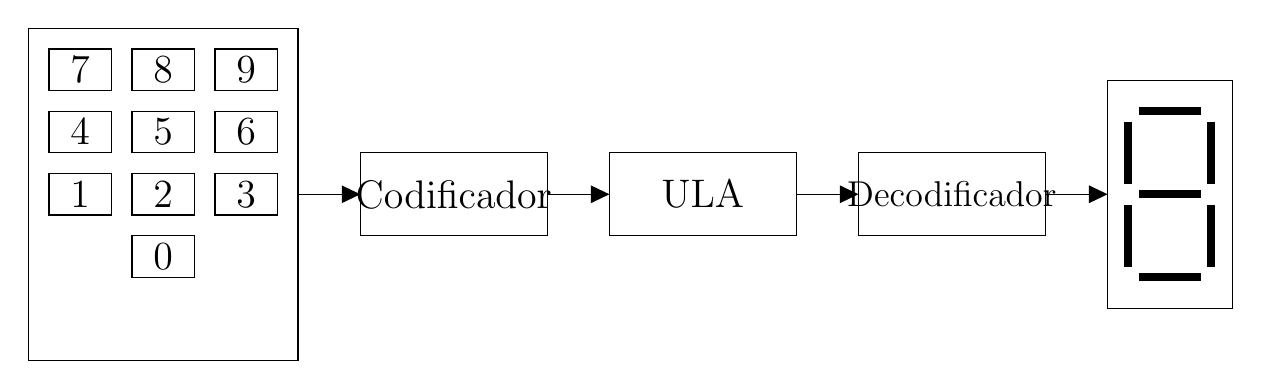
\begin{tikzpicture}[x=0.75pt,y=0.75pt,yscale=-1,xscale=1]
%uncomment if require: \path (0,300); %set diagram left start at 0, and has height of 300

%Shape: Rectangle [id:dp8798188650405219] 
\draw   (30,50) -- (160,50) -- (160,210) -- (30,210) -- cycle ;
%Shape: Rectangle [id:dp593444354888008] 
\draw   (40,60) -- (70,60) -- (70,80) -- (40,80) -- cycle ;
%Shape: Rectangle [id:dp4412846627526852] 
\draw   (80,60) -- (110,60) -- (110,80) -- (80,80) -- cycle ;
%Shape: Rectangle [id:dp2343273962035186] 
\draw   (120,60) -- (150,60) -- (150,80) -- (120,80) -- cycle ;
%Shape: Rectangle [id:dp05777918912875246] 
\draw   (40,90) -- (70,90) -- (70,110) -- (40,110) -- cycle ;
%Shape: Rectangle [id:dp9955010424516375] 
\draw   (80,90) -- (110,90) -- (110,110) -- (80,110) -- cycle ;
%Shape: Rectangle [id:dp24021539717259266] 
\draw   (120,90) -- (150,90) -- (150,110) -- (120,110) -- cycle ;
%Shape: Rectangle [id:dp36169684584711925] 
\draw   (40,120) -- (70,120) -- (70,140) -- (40,140) -- cycle ;
%Shape: Rectangle [id:dp7232437677097003] 
\draw   (80,120) -- (110,120) -- (110,140) -- (80,140) -- cycle ;
%Shape: Rectangle [id:dp6884539525496838] 
\draw   (120,120) -- (150,120) -- (150,140) -- (120,140) -- cycle ;
%Shape: Rectangle [id:dp9961423077173726] 
\draw   (80,150) -- (110,150) -- (110,170) -- (80,170) -- cycle ;
%Shape: Rectangle [id:dp6643057105712631] 
\draw   (190,110) -- (280,110) -- (280,150) -- (190,150) -- cycle ;
%Shape: Rectangle [id:dp7094011053258715] 
\draw   (550,75) -- (610,75) -- (610,185) -- (550,185) -- cycle ;
%Shape: Rectangle [id:dp2693438921699036] 
\draw   (310,110) -- (400,110) -- (400,150) -- (310,150) -- cycle ;
%Shape: Rectangle [id:dp3654960401722005] 
\draw   (430,110) -- (520,110) -- (520,150) -- (430,150) -- cycle ;
%Straight Lines [id:da6667328032348829] 
\draw    (160,130) -- (188,130) ;
\draw [shift={(190,130)}, rotate = 180] [fill={rgb, 255:red, 0; green, 0; blue, 0 }  ][line width=0.75]  [draw opacity=0] (8.93,-4.29) -- (0,0) -- (8.93,4.29) -- cycle    ;

%Straight Lines [id:da5165651690517046] 
\draw    (280,130) -- (308,130) ;
\draw [shift={(310,130)}, rotate = 180] [fill={rgb, 255:red, 0; green, 0; blue, 0 }  ][line width=0.75]  [draw opacity=0] (8.93,-4.29) -- (0,0) -- (8.93,4.29) -- cycle    ;

%Straight Lines [id:da17751850693095572] 
\draw    (400,130) -- (428,130) ;
\draw [shift={(430,130)}, rotate = 180] [fill={rgb, 255:red, 0; green, 0; blue, 0 }  ][line width=0.75]  [draw opacity=0] (8.93,-4.29) -- (0,0) -- (8.93,4.29) -- cycle    ;

%Straight Lines [id:da4998570413390182] 
\draw [color={rgb, 255:red, 0; green, 0; blue, 0 }  ,draw opacity=1 ][line width=3]    (560,95) -- (560,125) ;


%Straight Lines [id:da05287212083080073] 
\draw [color={rgb, 255:red, 0; green, 0; blue, 0 }  ,draw opacity=1 ][line width=3]    (600,95) -- (600,125) ;


%Straight Lines [id:da9146969001147236] 
\draw [color={rgb, 255:red, 0; green, 0; blue, 0 }  ,draw opacity=1 ][line width=3]    (560,135) -- (560,165) ;


%Straight Lines [id:da37610179690179124] 
\draw [color={rgb, 255:red, 0; green, 0; blue, 0 }  ,draw opacity=1 ][line width=3]    (600,135) -- (600,165) ;


%Straight Lines [id:da2798262228013664] 
\draw [color={rgb, 255:red, 0; green, 0; blue, 0 }  ,draw opacity=1 ][line width=3]    (595,130) -- (565,130) ;


%Straight Lines [id:da15184615547446478] 
\draw [color={rgb, 255:red, 0; green, 0; blue, 0 }  ,draw opacity=1 ][line width=3]    (595,90) -- (565,90) ;


%Straight Lines [id:da20609816632014244] 
\draw [color={rgb, 255:red, 0; green, 0; blue, 0 }  ,draw opacity=1 ][line width=3]    (595,170) -- (565,170) ;


%Straight Lines [id:da16937059284664002] 
\draw    (520,130) -- (548,130) ;
\draw [shift={(550,130)}, rotate = 180] [fill={rgb, 255:red, 0; green, 0; blue, 0 }  ][line width=0.75]  [draw opacity=0] (8.93,-4.29) -- (0,0) -- (8.93,4.29) -- cycle    ;


% Text Node
\draw (135,70) node   {\Large $9$};
% Text Node
\draw (95,70) node   {\Large $8$};
% Text Node
\draw (55,70) node   {\Large $7$};
% Text Node
\draw (135,100) node   {\Large $6$};
% Text Node
\draw (135,130) node   {\Large $3$};
% Text Node
\draw (95,160) node   {\Large $0$};
% Text Node
\draw (95,130) node   {\Large $2$};
% Text Node
\draw (95,100) node   {\Large $5$};
% Text Node
\draw (55,100) node   {\Large $4$};
% Text Node
\draw (55,130) node   {\Large $1$};
% Text Node
\draw (235,130) node  [align=left] {\Large Codificador};
% Text Node
\draw (355,130) node  [align=left] {\Large ULA};
% Text Node
\draw (475,130) node [scale=0.9] [align=left] {\Large Decodificador};


\end{tikzpicture}
}
\end{frame}

\begin{frame}{Realimentação de variáveis de estado}
\begin{block}{Introdução}
	Realimentando o sistema a partir da saída temos:
\end{block}
\vspace{0,1 cm}
\centering
\scalebox{.8}{\deftkzbds
	
\begin{tikzpicture}[auto, node distance=2cm,>=Latex]
	
	\node [input, name=input] {};
	
	\node [coordinate, right=of input] (junction) {};
	\draw (input) -- node[near start] {$E(z)$} (junction);
	
	\node [block, right=of junction] (ei) {$ C_i(z) $};
	\node [block, above=of ei] (kp) {$ C_p(z) $};
	\node [block, below=of ei] (cd) {$ C_d(z) $};
	
	\draw [->] (junction) -- (ei);
	\draw [->] (junction) |- (kp);
	\draw [->] (junction) |- (cd);
	
	\node [sum, right=2cm of ei] (sum) {$ \phantom{\sum} $};
	\draw (sum) ++(-8pt,-8pt) -- ++(16pt,16pt) ++(-16pt,0pt) -- +(16pt,-16pt);
	
	\draw [<-] (sum) -- node[very near start, above] {$ + $} (ei);
	\draw [<-] (sum) |- node[very near start, right] {$ + $} (kp);
	\draw [<-] (sum) |- node[very near start, left] {$ + $} (cd);
	
	\node [output, right=of sum] (output) {};
	\draw [->] (sum) -- node[near end] {$ U(z) $} (output);
\end{tikzpicture}}
\end{frame}

\begin{frame}{Realimentação de variáveis de estado}
\begin{block}{Introdução}
	\begin{itemize} 
	\item Considerando\\
	$$ G(z) = \dfrac{z}{(z-1)(z-0,9)}$$
	\item A equação característica é:\\
	$$ z^2 + (K_0 - 1,9)z + 0,9 = 0 $$
	\item Alterando o parâmetro $ K_0 $, não é possível definir de forma arbitrária a \textbf{equação característica}, pois só existe uma variável livre $ K_0 $, para dois coeficientes da equação característica.
	$$ \bm{u} = r - K_0\bm{y} $$
	\end{itemize}
\end{block}
\end{frame}

\begin{frame}{Realimentação de variáveis de estado}
\begin{block}{Introdução}
	"O princípio de que as entradas devem ser computadas utilizando o \textbf{estado} foi anunciado e enfatizado por Richard Ballman em meados da década de 1950. \textbf{Essa é a ideia fundamental do controle realimentado}."
	\begin{flushright}
		(Kalman, 1960)
	\end{flushright}
	\begin{itemize}
		\item Partindo desse conceito, Kalman iniciou sua análise considerando uma lei de controle no seguinte formato
		$$ \bm{u}(kT) = \mathcal{X}\left ( \bm{x}(kT), kT\right ) $$
		\item Simplificando posteriormente
		\begin{align*}
		\bm{u}(kT) = -K\bm{x}(kT), \quad  & \bm{x} \in \mathbb{R}^n \\ 
		& K \in \mathbb{R}^{1 \times n}
		\end{align*}
	\end{itemize}
\end{block}
\end{frame}

\begin{frame}{Realimentação de variáveis de estado}
\vspace{0,1 cm}
\begin{center}
	Sistema com realimentação de estados\\
	\scalebox{.8}{%\begin{tikzpicture}[scale=1.5,>=latex, every node/.style={inner sep=2pt}]
%	
%	%\draw[pattern=north west lines, draw=mWhite] (0cm,0cm) circle(1cm);
%
%	\draw[dashed] (0cm,0cm) circle(1cm);
%	
%    % draw the coordinates
%    \draw[->, fill=white] (-1.5cm,0cm) -- (1.5cm,0cm) node[right=2pt] {$\Re(z)$};
%    \draw[->, fill=white] (0cm,-1.5cm) -- (0cm,1.5cm) node[above=2pt] {$\Im(z)$};
%    
%    \draw[->] (0,0) -- (45:1) node[right=2pt] {$ r=1 $};
%    
%    \draw[] (-1.4,0) ++(-2pt,-2pt) -- ++(4pt,4pt) ++(-4pt,0pt) -- ++(4pt,-4pt) +(-2pt,2pt) node[below=2pt, xshift=-3pt] {$ -1,4 $};
%    
%    \draw[fill=white] (-0.25,0) circle (1pt) node[below=2pt, xshift=-3pt] {$ -0,25 $};
%    
%    \draw[fill=white] (0,0) circle (1pt) node[below right=2pt] {$ 0 $};
%    
%    \draw[] (0.6,0) ++(-2pt,-2pt) -- ++(4pt,4pt) ++(-4pt,0pt) -- ++(4pt,-4pt) +(-2pt,2pt) node[below=2pt] {$ 0,6 $};
%\end{tikzpicture}


\begin{tikzpicture}[scale=1.5,>=latex, every node/.style={inner sep=2pt}]

\draw[pattern=south east lines, draw=mWhite] (0cm,0cm) circle(1.4cm);

\draw[dashed] (0cm,0cm) circle(1.4cm);

\draw[dashed, fill=white] (0cm,0cm) circle(0.6cm);

% draw the coordinates
\draw[->, fill=white] (-2cm,0cm) -- (2cm,0cm) node[right=2pt,fill=white] {$\Re(z)$};
\draw[->, fill=white] (0cm,-2cm) -- (0cm,2cm) node[above=2pt,fill=white] {$\Im(z)$};

%\draw[fill=black] (-1.4,0) ++(-2pt,-2pt) -- ++(4pt,4pt) ++(-4pt,0pt) -- ++(4pt,-4pt) +(-2pt,2pt) node[below left=2pt] {$ -1,4 $};

\node[below left=2pt] at (-1.4,0) {$ -1,4 $};

%    \draw[fill=black] (-0.6,0) circle (1pt) node[below=2pt,fill=mWhite] {$ -0,6 $};

%\draw[fill=black] (0.6,0) ++(-2pt,-2pt) -- ++(4pt,4pt) ++(-4pt,0pt) -- ++(4pt,-4pt) +(-2pt,2pt) node[below left=2pt] {$ 0,6 $};

\node[below left=2pt] at (0.6,0) {$ 0,6 $};

%    \draw[fill=black] (1.4,0) circle (1pt) node[below=2pt,fill=mWhite] {$ 1,4$};

	\draw[->,line width=1.2pt,white] (0,0) -- (45:1);
	\draw[->,thick] (0,0) -- (45:1) node[left,rotate=45,near start,below,xshift=2pt,yshift=1pt] {\tiny$ r=1 $};
	
	\draw[line width=1.2pt,white] (0cm,0cm) circle(1cm);
	\draw[densely dashed,thick] (0cm,0cm) circle(1cm);
\end{tikzpicture}}
\end{center}
\end{frame}

\begin{frame}{Realimentação de variáveis de estado}
\begin{block}{Introdução}
\begin{itemize}
    \item Visto que os polos determinam a \textbf{dinâmica} de um sistema, um sistema realimentado tem a capacidade de \textbf{alterar a localização dos polos} do sistema controlado e, portanto, tem o potencial de mudar  a dinâmica original.
    \item Esta capacidade de alocação de polos está intrinsecamente ligada ao número de parâmetros livres que o controlador possui.
    \item A \textbf{alocação de polos} permite o controle de sistemas de múltiplas entradas e múltiplas saídas. A ideia principal é \textbf{realimentar todas as variáveis de estado}, por meio do vetor $\bm{x}$, em vez de fazer a realimentação com o vetor de saída $\bm{y}$.
\end{itemize}
\end{block}
\end{frame}

\begin{frame}{Realimentação de variáveis de estado}
\begin{block}{Formulação matemática}
\begin{itemize}
    \item Considere a lei de controle
\end{itemize}
\begin{align*}
    \bm{u}(k) &= r(k) - k_1x_1(k) - k_2x_2(k) - ... - k_nx_n(k) \\
    &= r(k) - K\bm{x}(k)
\end{align*}
\vspace{-0.3cm}
\begin{itemize}
    \item[] em que $K = \begin{bmatrix}
    k_1 & k_2 & \cdots & k_n
    \end{bmatrix}$
    \item Neste esquema, cada variável de estado é realimentada por meio de um ganho, representado pelo vetor de realimentação $K$. Esta técnica permite a \textbf{alocação dos polos nas posições desejadas}, desde que o sistema seja controlável.
\end{itemize}
\begin{align*}
    \bm{x}(k+1) &= A\bm{x}(k) + B\bm{u}(k) \\
    &= A\bm{x}(k) + B[r(k) - K\bm{x}(k)] \\
    &= (A - BK)\bm{x}(k) + Br(k)
\end{align*}
\end{block}
\end{frame}

\begin{frame}{Realimentação de variáveis de estado}
\begin{block}{Equação característica do sistema realimentado}
\begin{itemize}
    \item A equação característica do sistema realimentado é dada por
\end{itemize}
$$\boxed{|\lambda I - (A-BK)| =  0}$$
\begin{itemize}
    \item Escrevendo o sistema na forma canônica controlável:
\end{itemize}
\begin{align*}
    BK = \begin{bmatrix}
    0 \\ 0 \\ \vdots \\ 0 \\ 1
    \end{bmatrix}
    \begin{bmatrix}
    k_1 & k_2 & \cdots & k_n
    \end{bmatrix} = \begin{bmatrix}
    0 & 0 & 0 & \cdots & 0 \\
    0 & 0 & 0 & \cdots & 0 \\
    \vdots & \vdots & \vdots & \ddots & \vdots \\
    0 & 0 & 0 & \cdots & 0 \\
    k_1 & k_2 & k_3 & \cdots & k_n
    \end{bmatrix}
\end{align*}
\end{block}
\end{frame}

\begin{frame}{Realimentação de variáveis de estado}
\begin{block}{Equação característica do sistema realimentado}
\vspace{0.3cm}
\begin{align*}
    A - BK &= \begin{bmatrix}
    0 & 1 & 0 & \cdots & 0 \\
    0 & 0 & 1 & \cdots & 0 \\
    \vdots & \vdots & \vdots & \ddots & \vdots \\
    0 & 0 & 0 & \cdots & 1 \\
    -a_0 & -a_1 & -a_2 & \cdots & -a_{n-1}
    \end{bmatrix} - \begin{bmatrix}
    0 & 0 & 0 & \cdots & 0 \\
    0 & 0 & 0 & \cdots & 0 \\
    \vdots & \vdots & \vdots & \ddots & \vdots \\
    0 & 0 & 0 & \cdots & 0 \\
    k_1 & k_2 & k_3 & \cdots & k_n
    \end{bmatrix} \\
    &= \begin{bmatrix}
    0 & 1 & 0 & \cdots & 0 \\
    0 & 0 & 1 & \cdots & 0 \\
    \vdots & \vdots & \vdots & \ddots & \vdots \\
    0 & 0 & 0 & \cdots & 1 \\
    -(a_0+k_1) & -(a_1+k_2) & -(a_2+k_3) & \cdots & -(a_{n-1}+k_n)
    \end{bmatrix}
\end{align*}
\end{block}
\end{frame}

\begin{frame}{Realimentação de variáveis de estado}
\begin{block}{Comparação entre os polinômios}
\begin{itemize}
    \item O polinômio característico do sistema é, portanto,
\end{itemize}
$$\Delta(\lambda) = \lambda^n + (a_{n-1}+k_n)\lambda^{n-1} + ... + (a_1+k_2)\lambda + (a_0+k_1)$$
\vspace{-0.3cm}
\begin{itemize}
    \item O polinômio característico desejado para o sistema em malha fechada é:
\end{itemize}
$$\Delta_d(\lambda) = \lambda^n + \alpha_{n-1}\lambda^{n-1} + ... + \alpha_1\lambda + \alpha_0$$
\vspace{-0.3cm}
\begin{itemize}
    \item Deste modo,
\end{itemize}
$$k_{i+1} = \alpha_i - a_i, \ i=0,1,...,n-1$$
\begin{itemize}
    \item Se o par $(A,B)$ for completamente controlável existe um vetor $K$ tal que os autovalores de $(A-BK)$ podem ser arbitrariamente \textbf{escolhidos}.
\end{itemize}
\end{block}
\end{frame}

\begin{frame}{Realimentação de variáveis de estado - Exemplo \#01}
\begin{block}{Problema}
	Encontrar um vetor de ganhos $K$ (\textit{caso haja}) tal que o sistema em malha fechada abaixo possua autovalores em $\lambda_1 = \num{0,8}$ e $\lambda_2 = \num{0,9}$.
	\begin{align*}
	\begin{bmatrix} x_1(k+1) \\ x_2(k+1) \end{bmatrix}
	&=
	\begin{bmatrix}
	0 & 1 \\ -\num{0,96} & -2
	\end{bmatrix}
	\begin{bmatrix}
	x_1(k) \\ x_2(k)
	\end{bmatrix}
	+
	\begin{bmatrix}
	0 \\ 1
	\end{bmatrix}
	u(k)
	\end{align*}
\end{block}
\end{frame}

\begin{frame}{Realimentação de variáveis de estado - Exemplo \#01}
\begin{block}{Resolução}
	\begin{itemize}
		\item O polinômio característico desejado para a malha fechada é:
	\end{itemize}
	$$\Delta_d(\lambda) = (\lambda-\num{0,8})(\lambda-\num{0,9}) = \lambda^2 - \num{1,7}\lambda + \num{0,72}$$
	\vspace{-0.3cm}
		\begin{itemize}
		\item A nova matriz dinâmica do sistema é dada por
	\end{itemize}
	$$ \tilde{A} = A - BK = \begin{bmatrix}
		0 & 1\\ 
		-\num{0,96} & -2
	\end{bmatrix} -
	\begin{bmatrix}
		0 & 0 \\ 
		K_1 & K_2 
	\end{bmatrix} =
	\begin{bmatrix}
		0 & 1\\ 
		-\num{0,96} - K_1 & -2 - K_2
	\end{bmatrix} $$
	\vspace{-0.2cm}
	\begin{itemize}
		\item A nova equação característica se torna:
	\end{itemize}
	$$ \Delta_{\tilde{A}} = \lambda^2 + (2 + K_2)\lambda + (\num{0,96} + K_1)$$
	\vspace{-0,3 cm}
	\begin{itemize}
		\item Por comparação de coeficientes podemos determinar os ganhos
	\end{itemize}
	$$ \num{0,96}+K_1 = \num{0,72} \therefore K_1 = -\num{0,24} $$
	$$ 2+K_2 = -\num{1,7} \therefore K_2 = -\num{3,7} $$
	$$K = \begin{bmatrix}
		-\num{0,24} & -\num{3,7}
	\end{bmatrix}$$
\end{block}
\end{frame}

\begin{frame}{Realimentação de variáveis de estado}
\begin{block}{A fórmula de Ackermann}
\begin{itemize}
    \item É possível determinar $K$ sem supor que $(A,B)$ esteja na forma canônica controlável, utilizando a \textbf{fórmula de Ackermann} (\textit{mesmo assim a condição é que o sistema seja totalmente  controlável, ou seja, $\rho[\mathcal{C}] = n$}).
\end{itemize}
$$\boxed{K = \begin{bmatrix}
    0 & 0 & \cdots & 0 & 1
    \end{bmatrix} \mathcal{C}^{-1}\Delta_d(A)}$$
\vspace{-0.3cm}
\begin{itemize}
    \item[] onde $\Delta_d(A)$ é o polinômio característico desejado para a malha fechada avaliado em $A \in \mathbb{R}^{n \times n}$, isto é,
\end{itemize}
\vspace{0.2cm}
$$\Delta_d(A) = A^n + \alpha_{n-1}A^{n-1} + ... + \alpha_1A + \alpha_0I$$
\end{block}
\end{frame}

\begin{frame}{Realimentação de variáveis de estado - Exemplo \#02}
\begin{block}{Problema}
Encontrar um vetor de ganhos $K$ (\textit{caso haja}) tal que o sistema em malha fechada abaixo possua autovalores em $\lambda_1 = \num{0,9}$ e $\lambda_2 = \num{0,8}$.
\begin{align*}
    \begin{bmatrix} x_1(k+1) \\ x_2(k+1) \end{bmatrix}
    &=
    \begin{bmatrix}
    -\num{1,2} & 1 \\ 0 & -\num{0,8}
    \end{bmatrix}
    \begin{bmatrix}
    x_1(k) \\ x_2(k)
    \end{bmatrix}
    +
    \begin{bmatrix}
    \num{0,5} \\ 1
    \end{bmatrix}
    u(k)
\end{align*}
\end{block}
\end{frame}

\begin{frame}{Realimentação de variáveis de estado - Exemplo \#02}
\begin{block}{Resolução}
\begin{itemize}
    \item O primeiro passo consiste em verificar a controlabilidade do sistema:
\end{itemize}
\begin{align*}
    \mathcal{C} &= \begin{bmatrix} B & AB \end{bmatrix} \\
    &= \begin{bmatrix} \num{0,5} & \num{0,4} \\ 1 & -\num{0,8} \end{bmatrix}
\end{align*}
\vspace{-0.3cm}
\begin{itemize}
    \item Calculando o determinante da matriz de controlabilidade, temos:
\end{itemize}
$$\text{det}[\mathcal{C}] = -\num{0,8} \neq 0 $$
Desta forma, o sistema é completamente controlável e $\rho = n = 2$.
\end{block}
\end{frame}

\begin{frame}{Realimentação de variáveis de estado - Exemplo \#02}
\begin{block}{Resolução}
\begin{itemize}
    \item O polinômio característico desejado para a malha fechada é:
\end{itemize}
$$\Delta_d(\lambda) = (\lambda-\num{0,9})(\lambda-\num{0,8}) = \lambda^2 - \num{1,7}\lambda + \num{0,72}$$
\vspace{-0.3cm}
\begin{itemize}
    \item O polinômio característico desejado para a malha fechada avaliado em $A \in \mathbb{R}^{n \times n}$ é:
\end{itemize}
\begin{align*}
    \lambda_d(A) &= \left(\begin{bmatrix}
    -\num{1,2} & 1 \\ 0 & -\num{0,8}
    \end{bmatrix}\right)^2 - \num{1,7} \begin{bmatrix}
    -\num{1,2} & 1 \\ 0 & -\num{0,8}
    \end{bmatrix} + \num{0,72}\begin{bmatrix}
    1 & 0 \\ 0 & 1
    \end{bmatrix} \\
    &= \begin{bmatrix}
    \num{4,2} & -\num{3,7} \\ 0 & \num{2,72}
    \end{bmatrix}
\end{align*}
\end{block}
\end{frame}

\begin{frame}{Realimentação de variáveis de estado - Exemplo \#02}
\begin{block}{Resolução}
\begin{itemize}
    \item Com isso, o vetor de ganhos $K$ é dado por
\end{itemize}
\begin{align*}
    K &= \begin{bmatrix}
    0 & 1
    \end{bmatrix} \mathcal{C}^{-1}\Delta_d(A) \\
    &= \begin{bmatrix}
    0 & 1
    \end{bmatrix} \begin{bmatrix} \num{0,5} & \num{0,4} \\ 1 & -\num{0,8} \end{bmatrix}^{-1} \begin{bmatrix}
    \num{4,2} & -\num{3,7} \\ 0 & \num{2,72}
    \end{bmatrix} \\
    &= \begin{bmatrix}
    0 & 1
    \end{bmatrix} \begin{bmatrix} 1 & \num{0,5} \\ \num{1,25} & -\num{0,625} \end{bmatrix} \begin{bmatrix}
    \num{4,2} & -\num{3,7} \\ 0 & \num{2,72}
    \end{bmatrix} \\
    &= \begin{bmatrix}
    \num{1,25} & -\num{0,625}
    \end{bmatrix}
    \begin{bmatrix}
    \num{4,2} & -\num{3,7} \\ 0 & \num{2,72}
    \end{bmatrix} \\
    &= \begin{bmatrix}
    \num{5,25} & -\num{6,325}
    \end{bmatrix}
\end{align*}
\end{block}
\end{frame}

\cprotect\frame{
\frametitle{\MATLAB}
\begin{block}{}
\begin{verbatim}
>>acker(A,B,roots(p)) 
\end{verbatim}
determina o vetor de ganhos $K$ utilizando a fórmula de Ackermann utilizando o par $\bm{(A,B)}$ e as raízes do polinômio característico desejado $\bm{p}$. \\
\vspace{0.2cm}
\textbf{Exemplo}: cálculo do exemplo \#01
\end{block}
\centerline{\includegraphics[width=0.45\linewidth]{Figuras/Ch15/fig4.PNG}}
}

\cprotect\frame{
\frametitle{\MATLAB}
\begin{block}{}
\begin{verbatim}
>>place(A,B,roots(p)) 
\end{verbatim}
determina o vetor de ganhos $K$ utilizando a realimentação de estados por meio do par $\bm{(A,B)}$ e as raízes do polinômio característico desejado $\bm{p}$. \\
\vspace{0.2cm}
\textbf{Exemplo}: cálculo do exemplo \#01
\end{block}
\centerline{\includegraphics[width=0.4\linewidth]{Figuras/Ch15/fig5.PNG}}
}

\cprotect\frame{
\frametitle{\MATLAB}
\begin{block}{}
\begin{itemize}
    \item \texttt{acker} só se aplica  ao caso monovariável, mas aceita polos com  multiplicidade maior que um. 
    \item \texttt{place} tem  propriedades numéricas melhores, pode ser usada no caso multivariável, mas não aceita  polos com multiplicidade maior que o número  de entradas.
\end{itemize}
\end{block}
}

\frame{
\frametitle{Exercícios}
\begin{block}{}
01. Verifique que $(A-BK)$ (\textit{do exemplo \#01 da realimentação de variáveis de estado}) de fato possui os autovalores desejados, ao ser utilizado o vetor de ganhos $K$.

\vspace{1cm}

02. Considere um sistema discreto representado pelo seguinte espaço de estados:
\begin{align*}
    \bm{x}(k+1) &= \begin{bmatrix}
    0 & 1 \\
    -2 & 3 \\
    \end{bmatrix}\bm{x}(k) +  \begin{bmatrix}
    0 \\
    1 \\  
    \end{bmatrix}\bm{u}(k) \\
    \bm{y}(k) &= \begin{bmatrix}
    0 & 1
    \end{bmatrix}\bm{x}(k) 
\end{align*}
    
\begin{enumerate}
    \item[(a)] Este sistema é controlável?
    \item[(b)] Este sistema é observável?
    \item[(c)] Compare os resultados pelo \MATLAB.
\end{enumerate}
\end{block}
}

\frame{
\frametitle{Exercícios}
\begin{block}{}
03. Um sistema em tempo discreto possui as seguintes matrizes na representação em espaço de estados:
\begin{align*}
    A= \begin{bmatrix}
    0 & 1 \\
    -1 & -2 \\
    \end{bmatrix} \qquad \qquad  B=\begin{bmatrix}
    1 & 0 \\
    0 & 1 \\  
    \end{bmatrix}
\end{align*}
    
Verifique se esse sistema é controlável e, em caso positivo, forneça $K$ tal que o sistema com a lei de controle $\bm{u} = -K\bm{x}$ tenha  autovalores em $\lambda_1 = \num{0,1}$ e $\lambda_2 = \num{0,2}$. Compare os resultados pelo \MATLAB.
\end{block}
}

\frame{
\frametitle{Referências e exercícios complementares}
\begin{itemize}
\item AGUIRRE, Luis A. Controle de Sistemas Amostrados, 1 ed. [s.n.], 2019.
\end{itemize}
\centering{\alert{Página 355 - \textbf{Capítulo 8}}} \\
\vspace{0.4cm}
\begin{itemize}
\item FRANKLIN, Gene F.; POWELL, J. David; WOLKMAN, Michael L. Digital Control of Dynamic Systems, 3 ed. Addison-Wesley, 1998.
\end{itemize}
\centering{\alert{Página 352 - \textbf{Capítulo 8}}} \\
}